\documentclass{sig-alternate-10pt}
%\documentclass[letterpaper,11pt]{article}
\usepackage{url}
%\usepackage{usenix,epsfig,endnotes}
%\usepackage{fullpage} 
\setlength{\textheight}{9.5in}
%\setlength{\textwidth}{6.75in}
%\setlength{\oddsidemargin}{-.125in}
\usepackage{graphicx}
%\usepackage{subfigure}
%\usepackage{ifpdf}
%\usepackage{multicol}
%\usepackage{amsmath, amssymb, amsthm}
%\usepackage{rotating}
%\onehalfspacing
%\newcommand{\tbd}[1]{[{\bf{#1}}]}
\newcommand{\tbd}[1]{}
\newcommand{\ie}{{\it i.e.}}
\newcommand{\eg}{{\it e.g.}}
\newcommand{\etc}{{\it etc.}}
\newcommand{\eat}[1]{}
%\renewcommand\bibname{}

%\setlength\topmargin{0in}
%\usepackage{verbatim}
%\usepackage[compact]{titlesec}
%\usepackage[small]{caption}
\usepackage{times}

\title{Correspondence Checking for Computer Networks \\
\Large{CS 263 Project Proposal \vspace{-25pt}}}

\author{Colin Scott\thanks{In collaboration with Andi
Wundsam and Scott Shenker}\vspace{-15pt}}

%        \begin{multicols}{2}{{\it Draft - Please do not distribute.}}\\
        
%\author{Paper \#69, 14 Pages}
\date{}
\begin{document}
    \maketitle
    \thispagestyle{empty}
% Outline:
%
%1 Problem formulation
%  1.1 Why is the problem important/relevant?
%  1.2 What are the main challenges in solving the problem?
%
%2 Approach
%  2.1 What is your approach? Briefly describe it
%  2.2 How is you approach different/similar from/to related work? You
%      don't need to be exhaustive here.
%
%3 Deliverables/milestones
%   3.1 What do you plan to accomplish by the end of the semester? What are the
%   metrics of success?
%   3.2 Do you plan to work on the project past the end of the semester?, and
%   if yes, what do you hope to accomplish by the end?
%   3.3 Specify measurable milestones by Oct. 26th
%  
%4 Any special needs for the project?
\section{Background}

In software-defined networking (SDN), computer networks are represented
as an abstract graph called a `view`: 
\begin{align*}
G^{view} = (V^{view}, E^{view})
\end{align*}

An example view is depicted in Figure \ref{fig:app_view}. Forwarding elements are
represented as internal vertices:
\begin{align*}
V_{fwd}^{view} = \{ v \in V^{view} |\text{ } degree(v) > 1 \}
\end{align*}

\begin{figure}[t]
    \hspace{-10pt}
    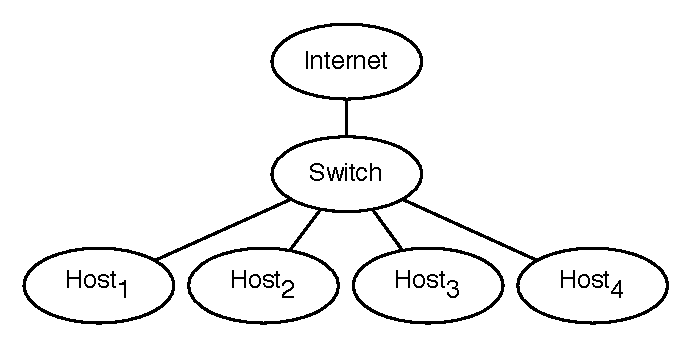
\includegraphics[width=3.25in]{../diagrams/necula_views/app_view.pdf}
    \caption[]{\label{fig:app_view} Example view. A single switch connects 
    four hosts and the rest of the Internet (modeled as a single vertex).} 
\end{figure}

End-hosts are represented as edge vertices:
\begin{align*}
V_{host}^{view} = \{ v \in V^{view} |\text{ } degree(v) = 1 \}
\end{align*}

End-hosts send and receive packets. A packet's source and destination,
among other information, is encoded in the packet's header:
\begin{align*}
h \in \{0,1\}^L = H
\end{align*}
where $L$ is the number of bits in
the header \cite{HeaderSpace}.

Upon receiving a packet, forwarding elements apply a transformation function:
\begin{align*}
T: (H_x \times E) \rightarrow (H_x \times E_{\emptyset})
\end{align*}
where $`x`$ denotes a wildcard bit, and $H_x = \{0,1,x\}^L$. We use $`\Psi`$ to denote the collection of all transfer functions.
Note that forwarding elements may rewrite fields of a packet header before passing it along. Forwarding elements may also drop packets,
in which case $T(.) = (.,\{\})$.

In this model, network traversal is simply a composition of transformation
functions. For example, if a header $h$ enters the network through edge
$e$, its state after $k$ hops will be:
\begin{align*}
\Phi^k(h,e) = \Psi(\Psi(\dots \Psi(h,e)\dots))
\end{align*}

In SDN, control programs specify the behavior of the network by defining
$\Psi^{view}$.

$G^{view}$ is simply a data-structure maintained by the SDN platform
(a software layer underneath the control program). The role of the platform
is to map $\Psi^{view}$ to
routing entries in the underlying forwarding elements of the
physical network. The physical network is also a graph:
\begin{align*}
G^{physical} = (V^{physical}, E^{physical}) \\
V_{fwd}^{physical} =  \{ v \in V^{physical} |\text{ } degree(v) > 1 \} \\
V_{host}^{physical} =  \{ v \in V^{physical} |\text{ } degree(v) = 1 \}
\end{align*}

Note that the mapping between $G^{view}$ and $G^{physical}$ is not
necessarily one-to-one; the SDN platform may virtualize the view
such that a single member of $V_{fwd}^{view}$ maps to multiple members of
$V_{fwd}^{physical}$. In general, the mapping from $G^{view}$ to
$G^{physical}$ can be represented as two functions:
\begin{align*}
f_{V} : V^{view} \rightarrow \mathcal{P}(V^{physical}) \\
f_{E} : E^{view} \rightarrow \mathcal{P}(E^{physical})
\end{align*}

A common pattern is to map a single forwarding element $v \in V_{fwd}^{view}$ to
an entire physical network $V_{fwd}^{physical}$. Figure \ref{fig:physical_view} depicts such a network.
As we will see later on, it is important to note that there is still a one-to-one correspondence
between $V_{host}^{view}$ and $V_{host}^{physical}$, as well as between the hosts' corresponding
access links, which we denote with:
\begin{align*}
E_{access}^{view} = \{ (e_1,e_2) \in E^{view} |\text{ } e_1 \in V_{host}^{view} \} \\
E_{access}^{physical} = \{ (e_1,e_2) \in E^{physical} |\text{ } e_1 \in V_{host}^{physical} \}
\end{align*}

Only end-hosts can insert new packets into the network. The
externally visible behavior of the network is therefore
the final location of all packet headers originating from an end-host:
\begin{align*}
\Omega: (H_{x} \times E_{access}) \rightarrow (H_{x} \times E_{\emptyset}) \\
\Omega(h,e) = \Phi^{\infty}(h,e)
\end{align*}

\begin{figure}[t]
    \hspace{-10pt}
    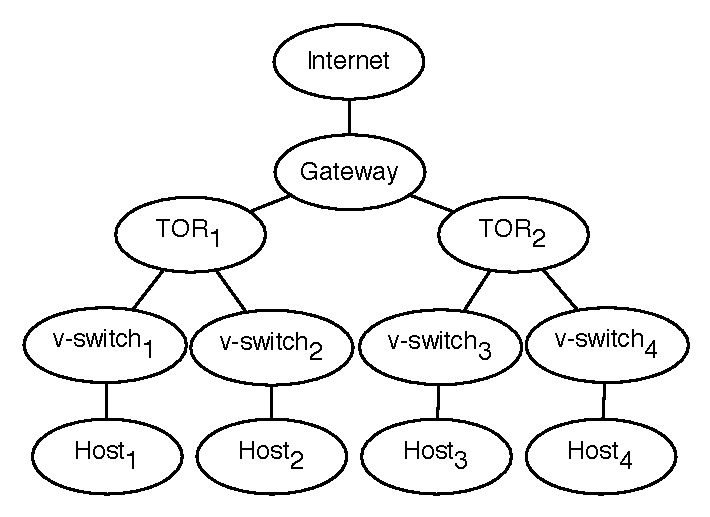
\includegraphics[width=3.25in]{../diagrams/necula_views/physical_view.pdf}
    \caption[]{\label{fig:physical_view} Example physical network. The four
    hosts from Figure \ref{fig:app_view} are each connected to a v-switch,
    which are in turn connected to top-of-rack switches, which are in turn
    connected to a single gateway router connected to the Internet.}
\end{figure}

\section{Problem Statement}

Ideally, it should always be the case that $\Omega^{view} = \Omega^{physical}$.
In practice however, there are often miscorrespondences between the two. Some
of these miscorrespondences are innocuous; networks are distributed systems,
and there are inevitable delays between updates in $G^{view}$ and the
corresponding changes in $G^{physical}$. Some miscorrespondences however are
due to critical bugs in the SDN platform. In general, the SDN platform is a
highly complex piece of software; it must deal with hardware-faults,
communication delays, and complex mapping functions $f_{V}$ and $f_{E}$. 
Moreover, production networks often contain $10's$ of thousands of
forwarding devices. In such an environment, the SDN control program must be
replicated across multiple servers to ensure scalability and fault-tolerance. 
The SDN platform must ensure that the view $G^{view}$ remains consistent
between all replicas, despite server failures and communication delays.

\section{Proposal}

I propose to design and built a mechanism for checking 
correspondence between $\Omega^{view}$ and $\Omega^{physical}$.
I plan to leverage techniques from model-checking \cite{symbolicmodel}.
In particular, my initial design will follow the approach in \cite{Anteater}:
\begin{enumerate}
\item Take a distributed snapshot of $G^{physical}$ \cite{distributedsnapshots}
\item Translate the routing tables of $V_{fwd}^{physical}$ into boolean
formulas
\item Do the same for $G^{view}$
\item Feed the boolean formulas to a SAT solver to identify
counterexamples:
\begin{align*}
 \{ (h,e) |\text{ } h \in H, e \in E^{view}_{access} \sim
 E^{physical}_{access}, \\
 \Omega^{view}(h,e) \neq  \Omega^{physical}(h,e) \}
\end{align*}
\end{enumerate}

I will implement my correspondence checker on top of the POX control platform
\cite{POX}.
I plan to submit this work, along with other aspects of my SDN debugger, to
OSDI 2012.

\scriptsize
\bibliographystyle{abbrv}
\bibliography{bib}

%\input{appendix}

\end{document}
